\documentclass[conference]{IEEEtran}
\IEEEoverridecommandlockouts
% IEEE conference template (IEEEtran.cls v1.8b, from ieee.org/conferences/publishing/templates)
% Prepared for the MAI-DRS 2026 workshop at IEEE BIBM 2026.
\usepackage{cite}
\usepackage{amsmath,amssymb,amsfonts}
\usepackage{graphicx}
\usepackage{textcomp}
\usepackage{xcolor}
\usepackage{booktabs}
\usepackage{url}
\usepackage[hidelinks]{hyperref}
\def\BibTeX{{\rm B\kern-.05em{\sc i\kern-.025em b}\kern-.08em T\kern-.1667em\lower.7ex\hbox{E}\kern-.125emX}}

% Set to 1 for an anonymised review copy, 0 for the named version.
\newif\ifanon
\anonfalse

\begin{document}

\title{Model-Class Mismatch and Aggregation Artifacts in Structure--Transcriptome Drug Repurposing}

\ifanon
\author{\IEEEauthorblockN{Anonymous Author(s)}
\IEEEauthorblockA{\textit{Affiliation withheld for review}}}
\else
\author{\IEEEauthorblockN{Rishik Kondadadi}
\IEEEauthorblockA{\textit{Eastview High School} \\
Apple Valley, MN, USA \\
rishik.kondadadi@gmail.com}
\IEEEauthorblockA{\textit{University of Minnesota} \\
Minneapolis, MN, USA \\
konda052@umn.edu}
\and
\IEEEauthorblockN{Dan McCreary}
\IEEEauthorblockA{\textit{Kelly-McCreary Associates} \\
Minneapolis, MN, USA \\
dan.mccreary@gmail.com}}
\fi

\maketitle

\begin{abstract}
Aligning drug chemical structure with perturbational transcriptomic response via
contrastive learning is an increasingly popular recipe for computational drug
repurposing. We evaluated it on real LINCS L1000 data across six pharmacological
drug classes and it failed: in every disease area a plain random forest on ECFP4
fingerprints beat every contrastive variant we trained ($p \le 0.027$), and it
also loses to four stronger structural baselines. The published alignment
objective this recipe comes from, reimplemented and tuned under the same
protocol, reaches $0.751$ against $0.917$ for the random forest and loses in all
six classes ($p \le 0.0039$). The more useful result is how
close we came to publishing the wrong explanation. Our initial analysis concluded
that L1000 expression carries essentially no usable drug-level signal (AUROC
$0.548$ on Phase~2, 95\% CI $[0.520, 0.577]$). Two ordinary choices produced that
number: averaging Level-5 signatures across all doses, cell lines and timepoints,
which cancels $64\%$ of signature magnitude, and using a random forest on the
resulting dense features. Correcting both reaches $0.752$ $[0.728, 0.776]$.
Because a chance-level result invites a strong conclusion, we tested the
explanation on an independent release (LINCS Phase~1, 46{,}726 signatures). Only
half of it survived. Model-class mismatch replicates: logistic regression beats
random forest by $+0.09$ to $+0.16$ in seven of eight release-by-representation
combinations. The aggregation effect does not, and reverses sign, with naive
averaging the \emph{best} representation on Phase~1 and the worst on Phase~2. We
report the failed half alongside the surviving half. Separately, even a correctly
specified expression arm stays redundant with structure (blend gain $+0.001$,
$p{=}0.15$), replicated on SIDER side-effect prediction, while gene-level analysis
confirms the corrected features encode real pharmacology, recovering HMGCR for
statins. We close with a self-audit of the defects behind these results, each of
which produced a publishable-looking but incorrect number.
\end{abstract}

\begin{IEEEkeywords}
drug repurposing, multi-modal learning, contrastive learning, LINCS L1000, transcriptomics, molecular fingerprints, negative results, reproducibility
\end{IEEEkeywords}


\section{Introduction}

Drug repurposing is an attractive target for machine learning: a repurposed
compound skips much of the cost and time of a new molecular entity. A natural
recipe, now widely instantiated, is to embed a drug's chemical structure and its
measured transcriptomic response into a shared space with a contrastive
objective, so that a disease signature can be matched against structurally
plausible candidates.

This paper reports that the recipe did not work in our hands, and argues that the
manner of its failure is more informative than the failure itself. Our
contributions are four negative or cautionary results, each accompanied by a
diagnosis:

\begin{enumerate}
    \item \textbf{The method loses to a trivial baseline.} Across six real
    pharmacological classes evaluated under a leak-free, drug-disjoint protocol,
    a random forest on raw ECFP4 fingerprints outperforms every contrastive
    variant we trained, in every class, and so do four stronger structural
    baselines. The published alignment objective of
    Finlayson et al.~\cite{finlayson2021}, reimplemented and tuned under the
    same protocol, loses in all six classes as well
    (Sections~\ref{sec:f1} to~\ref{sec:published}).

    \item \textbf{Two ordinary choices produced a chance-level result.} Naive
    signature aggregation and an ill-suited downstream model class together left
    the expression modality at $0.548$ on Phase~2 (95\% CI $[0.520, 0.577]$).
    Correcting both reached $0.752$ $[0.728, 0.776]$ (Section~\ref{sec:f2}).

    \item \textbf{Only half of that explanation replicates.} On LINCS Phase~1
    the model-class effect holds at $+0.09$ to $+0.16$ across representations,
    while the aggregation effect reverses sign. We report the failed half
    (Section~\ref{sec:repl}).

    \item \textbf{Correctly specified, the second modality is redundant.} With
    the expression arm properly constructed, blending still fails to improve on
    structure alone ($+0.001$, $p{=}0.15$), replicated on a second task family
    (Section~\ref{sec:f3}). Gene-level analysis confirms the corrected features
    nonetheless encode real pharmacology (Section~\ref{sec:bio}).
\end{enumerate}

We additionally report a self-audit (Section~\ref{sec:audit}) of four defects we
found in our own pipeline over the course of this work. We include it because
each defect produced a result that looked publishable, and because the
sequence illustrates a failure mode that is difficult to catch from the outside:
a chain of analyses that appear to be independent confirmations while all
sharing a single upstream defect.

\section{Related work}

\textbf{Contrastive alignment of molecules and transcriptomes.} Pairing chemical
structure with perturbational expression under a joint contrastive objective was
introduced by Finlayson et al.~\cite{finlayson2021}, who also flagged generalisation across cell
lines and compounds as unresolved. The CLIP formulation~\cite{radford2021} that most such work adapts, and the alignment and uniformity
diagnostics of Wang and Isola~\cite{wang2020}, are the two pieces of contrastive machinery we
use directly. Subsequent work has applied contrastive objectives to
drug-disease association tables and biomedical knowledge graphs, generally
reporting favourable within-benchmark results.

\textbf{Known problems with L1000 signal.} Our diagnosis rests on findings that
are individually established. Sirci et al.~\cite{sirci2017} report that a majority of CMap
compounds produce weak transcriptional responses and that class recovery for
those compounds is close to random, recommending that high-variability compounds
be discarded. Lim and Pavlidis~\cite{lin2021} document limited cross-version reproducibility of
L1000 differential expression, with reproducibility depending strongly on
differential-expression strength. What we add is the observation that these
known properties interact with an ordinary preprocessing default to produce a
chance-level result that looks like a modality limit.

\textbf{Reported baselines near chance.} Published raw-signature baselines in
this area sometimes sit at or near $0.50$. We do not claim that any specific
published number arises from the mechanism we describe, and our own interval
does not contain the values we cite. The point is narrower: a chance-level
signature baseline is consistent with a preprocessing artifact, and the
possibility is worth excluding before such a number is interpreted as evidence
about the assay.

\ifanon
\textbf{Prior work in this line.} Deep learning has been applied to epilepsy drug
repurposing on LINCS data~\cite{kondadadi2025ctdn}, using a temporal-diffusion
architecture and reporting favourable results against published baselines. That
work used the naive drug-level signature aggregation we identify here as
problematic, and it has not been re-evaluated under the corrected pipeline. We
single it out because the failure mode described here applies to prior results in
this line as much as to the method we set out to test.
\else
\textbf{Our own prior work in this line.} One of us previously applied deep
learning to epilepsy drug repurposing on LINCS data~\cite{kondadadi2025ctdn},
using a temporal-diffusion architecture and reporting favourable results against
published baselines. That work used the naive drug-level signature aggregation
we identify here as problematic, and we have not re-evaluated it under the
corrected pipeline. We single it out because the failure mode described here
applies to our own earlier results as much as to the method we set out to test.
\fi

\textbf{Negative results in machine learning for biology.} The genre this paper
belongs to has an established rationale. Publication of successful pipelines alone
biases the field's estimate of what works, and diagnosing why an approach failed
is often more transferable than the approach itself would have been. Our
self-audit in Section~\ref{sec:audit} is written in that spirit.

\section{Setup}
\label{sec:setup}

\textbf{Data.} LINCS L1000 Phase~2 (GSE70138) Level-5 signatures over $978$
landmark genes, restricted to compound perturbations: $107{,}404$ signatures over
$1{,}768$ compounds and $30$ cell lines. Canonical SMILES were resolved via
PubChem for $1{,}725/1{,}768$ compounds ($97.6\%$); all yielded valid $2048$-bit
ECFP4 fingerprints (RDKit, radius~2), retaining $103{,}989$ signatures. Official
LINCS signature QC metrics (\texttt{tas}, \texttt{distil\_cc\_q75},
\texttt{distil\_ss}, \texttt{pct\_self\_rank\_q25}) were obtained from the GEO
supplementary \texttt{sig\_metrics} file.

\textbf{Labels.} Six pharmacologically standard, mutually exclusive drug classes
matched by compound name: antiepileptics (16 drugs), statins (5), SSRIs (6),
NSAIDs (8), beta-blockers (6), antipsychotics (7). Positive counts are small,
which is why we evaluate by repeated subsampling rather than a single split. A
second task family, SIDER side-effect prediction, is used for replication
(Section~\ref{sec:f3}); $534$ of our compounds map to SIDER, yielding $586$
side-effect endpoints with at least $25$ positive and $25$ negative drugs each.
The analyses in Section~\ref{sec:f3} use subsets of $40$ to $60$ of these.

\textbf{Protocol.} Repeated Monte-Carlo \emph{drug-disjoint} subsampling: for each
of $10$ seeds we hold out $\max(2, 35\%)$ of a class's positive drugs plus $150$
random negative drugs; no drug's signatures ever appear in both the fitting and
evaluation pools. Contrastive models use a CLIP-style symmetric InfoNCE objective
between a structure encoder (ECFP4 $\to$ 256-d) and an expression encoder
(978-d $\to$ 256-d), both 3-layer MLPs, learnable temperature; all in-batch pairs
sharing a drug identity are treated as positives. Each pretraining regime is run
with 3 independent seeds. Significance is Wilcoxon signed-rank, paired by
subsampling seed after averaging over pretraining seeds.

\section{Failure 1: the method loses to a trivial baseline}
\label{sec:f1}

Table~\ref{tab:main} reports downstream class recovery. A random forest on raw
ECFP4 fingerprints is the strongest method in all six classes, beating the
contrastive model by margins of $0.03$ to $0.42$ AUROC, significant in every case
($p \le 0.027$). The raw-concatenation baseline (structure $+$ expression
features fed jointly to one model) is \emph{worse} than structure alone in all
six classes, an early hint of the interference we diagnose in
Section~\ref{sec:f2}.

\begin{figure*}[t]
\centering
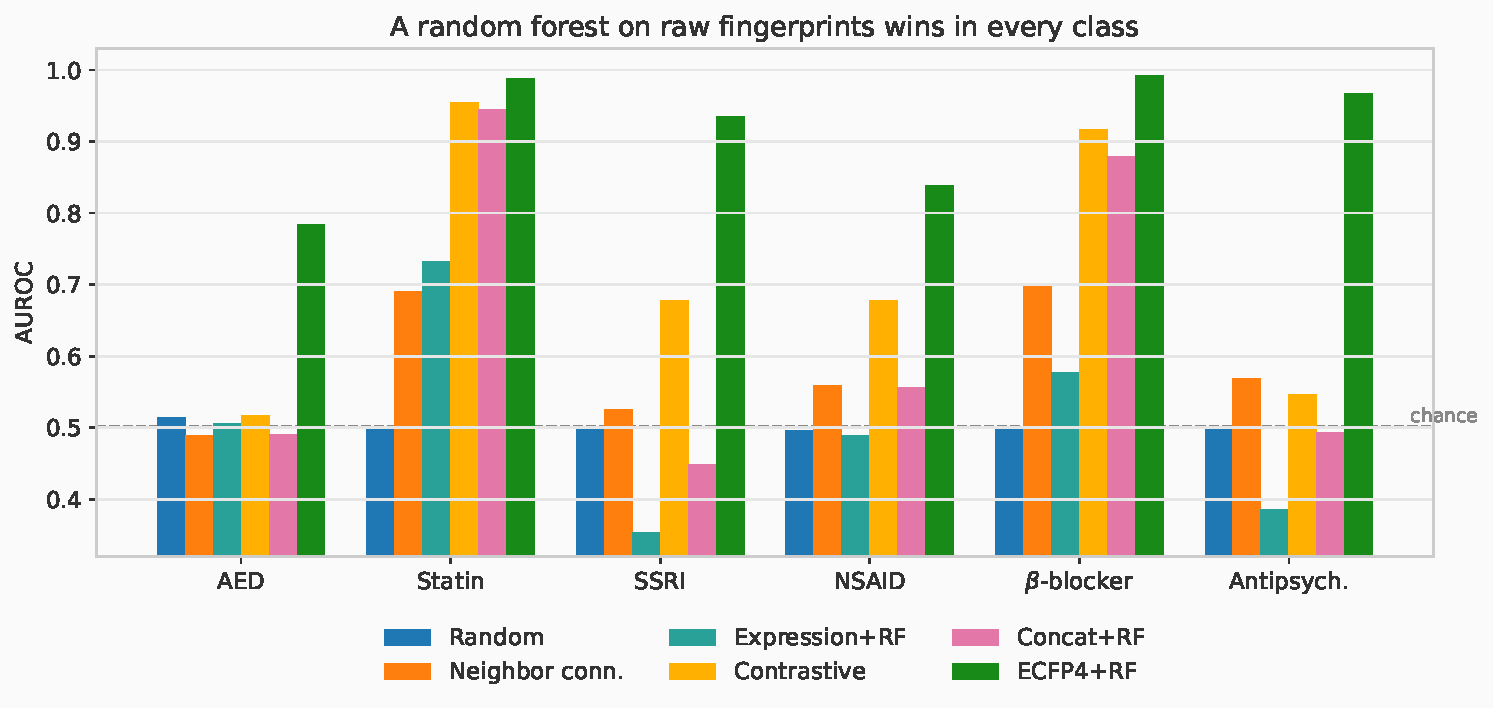
\includegraphics[width=0.82\textwidth]{../figures/fig2_methods.pdf}
\caption{Downstream class recovery across six pharmacological classes. The
contrastive model is beaten by a random forest on raw ECFP4 fingerprints in every
class. Note also that naively concatenating expression features to structure
(\emph{Concat+RF}) is \emph{worse} than structure alone in all six classes.}
\label{fig:methods}
\end{figure*}

\begin{table*}[t]
\centering\small
\caption{Downstream class recovery, mean AUROC over 10 drug-disjoint subsampling
seeds. Contrastive uses full-data pretraining, concatenated probe. A random
forest on raw fingerprints wins in every class.}
\label{tab:main}
\begin{tabular}{lcccccc}
\toprule
Method & AED & Statin & SSRI & NSAID & $\beta$-blocker & Antipsych. \\
\midrule
Random & 0.515 & 0.500 & 0.500 & 0.496 & 0.500 & 0.500 \\
Neighbor connectivity (param.-free) & 0.489 & 0.690 & 0.526 & 0.559 & 0.700 & 0.569 \\
Raw expression + RF & 0.506 & 0.733 & 0.353 & 0.490 & 0.577 & 0.386 \\
Raw concat + RF & 0.490 & 0.944 & 0.448 & 0.556 & 0.879 & 0.494 \\
Contrastive (full, concat) & 0.518 & 0.954 & 0.678 & 0.678 & 0.916 & 0.546 \\
\textbf{Raw ECFP4 + RF} & \textbf{0.784} & \textbf{0.987} & \textbf{0.935} & \textbf{0.838} & \textbf{0.992} & \textbf{0.968} \\
\bottomrule
\end{tabular}
\end{table*}

\subsection{The result holds against stronger structural baselines}
\label{sec:strong}

A random forest on ECFP4 is a simple comparator, and the natural objection is
that we chose an easy target. We therefore added four stronger structural
methods: a multi-representation random forest combining ECFP4 with MACCS keys
and ten physicochemical descriptors; gradient boosting on the same
representation; a Tanimoto-similarity $k$-nearest-neighbour scorer, the classic
chemoinformatics approach; and a logistic model on a Tanimoto kernel, which is
the structural analogue of the Gaussian interaction profile kernels that dominate
the drug-disease association literature.

\begin{table}[t]
\centering\small
\caption{Stronger structural baselines, mean AUROC over six classes and 10
drug-disjoint subsampling seeds. The richer representation beats our original
comparator, so the contrastive model loses to a stronger target than the one
reported in Table~\ref{tab:main}.}
\label{tab:strong}
\setlength{\tabcolsep}{4pt}
\begin{tabular}{lc}
\toprule
Method & Mean AUROC \\
\midrule
MACCS $+$ descriptors $+$ ECFP4, random forest & \textbf{0.931} \\
ECFP4, random forest & 0.917 \\
Tanimoto kernel, logistic regression & 0.910 \\
Tanimoto-similarity $k$NN & 0.903 \\
Multi-representation gradient boosting & 0.581 \\
\midrule
Finlayson et al.\ quadruplet alignment~\cite{finlayson2021} & 0.751 \\
Contrastive (full, concat) & 0.715 \\
\bottomrule
\end{tabular}
\end{table}

Combining fingerprints with MACCS keys and descriptors reaches $0.931$, above
the $0.917$ of the ECFP4 model we report throughout. The kernel and
nearest-neighbour methods land at $0.910$ and $0.903$. Gradient boosting at
default settings is the one poor performer ($0.581$), which we attribute to
overfitting a 2{,}225-dimensional representation with as few as five positive
compounds; we report it rather than tuning it away.

The conclusion is unchanged and slightly strengthened. Our contrastive model
does not merely lose to a convenient baseline. It loses to every reasonable
structural method we tried, including the kernel formulation that this
literature treats as standard.

\subsection{The published alignment objective loses as well}
\label{sec:published}

The sharper objection is that our contrastive model is our own, so its failure
might be a property of our implementation. We therefore reimplemented the
alignment objective of Finlayson et al.~\cite{finlayson2021}, the work that
introduced this recipe, from their Section~3.3: the adaptive-margin quadruplet
loss over all four cross-modal pairs of two matched structure-expression pairs,
a self-normalising expression encoder, and distance-weighted negative sampling
over compounds. No code accompanies that paper. We hold the structural input at
ECFP4 rather than their Chemprop D-MPNN so that what differs between the two
aligners is the objective and not the featurisation, and we give it the same
25-epoch budget, the same splits and the same downstream probe. The margin
parameters $\alpha$ and $\beta$ were selected over a $3 \times 6$ grid by
cross-modal retrieval MRR on a held-out fifth of the training compounds, never
on the evaluation drugs.

It does better than our own aligner and still loses. Mean AUROC over the six
classes is $0.751$ against $0.715$ for our CLIP-style model, so the published
objective is the stronger of the two contrastive methods and our comparison is
not resting on a weak stand-in. A random forest on ECFP4 beats it in all six
classes, every one significant at $p \le 0.0039$: AED $0.576$ against $0.784$,
statins $0.930$ against $0.987$, SSRIs $0.650$ against $0.935$, NSAIDs $0.752$
against $0.838$, beta-blockers $0.901$ against $0.992$, antipsychotics $0.697$
against $0.968$. All four stronger structural baselines beat it too.

Two deviations from the published description are worth stating. The
substitution of ECFP4 for the D-MPNN means we test their objective rather than
their full system, so a graph encoder could recover some of the gap. And their
negative sampler uses Wu et al.'s closed-form distance density, which assumes
points spread uniformly on a sphere; drug-level mean expression is not, and the
analytic form collapses the sampler onto each anchor's two nearest compounds, so
we substituted the empirical density of the observed distances.

\section{Failure 2: two ordinary choices that zero out a modality}
\label{sec:f2}

Our first reading of Table~\ref{tab:main} was that L1000 expression simply carries
no drug-level signal: expression-only averages $0.507$ over the six classes,
indistinguishable from the random control. We now believe that reading was wrong, and that the path to it is
the most transferable finding in this paper.

\textbf{Aggregation.} To obtain one feature vector per drug we had averaged all of
a compound's Level-5 signatures across doses, cell lines, and timepoints. This is
an unremarkable default. It is also destructive: the median norm of a drug's
averaged signature is $11.3$ versus $31.3$ for its individual signatures, i.e.\
averaging cancels $64\%$ of signature magnitude. The data are not the problem:
$99.9\%$ of compounds have at least one strongly active signature ($\ge 50$
landmark genes at $|z| > 2$), and only $7.8\%$ of individual signatures are weak
in the sense of carrying fewer than $25$ such genes.
At 30 subsampling repeats, aggregation alone moves expression-only AUROC from
$0.548$ to $0.635$ with the model held fixed at RF (Table~\ref{tab:corners});
the 6-repeat grid in Figure~\ref{fig:grid} puts the same shift at $0.525$ to
$0.619$. Figure~\ref{fig:cancel} shows the cancellation directly.

\textbf{Model class.} Independently, we had used a random forest for the
expression arm, mirroring the structure arm. Random forests are poorly matched to
dense, high-dimensional, low-sample expression features. Logistic regression on
the \emph{same} naively aggregated features reaches $0.663$ $[0.637, 0.689]$
where the random forest reaches $0.548$ $[0.520, 0.577]$. Structure, by contrast,
is model-robust (RF $0.9171$ vs.\ LogReg $0.9169$), so the choice penalises only
one arm.

\textbf{The conjunction.} Either choice alone leaves substantial signal; both
together leave the modality barely distinguishable from chance. The best cell
(high-dose aggregation $+$ logistic regression) reaches $0.752$ $[0.728, 0.776]$.
Table~\ref{tab:corners} collects the four corner estimates, each at 30
subsampling repeats ($n{=}180$) with bootstrap intervals. Every corner value
quoted in this paper comes from that table. The full grid in
Figure~\ref{fig:grid} and the Phase~2 columns of Table~\ref{tab:repl} use 6
repeats per cell and are intended to show the \emph{pattern} across the design
space rather than a precise level for any single cell. The three values this
paper reports for the naive-mean random-forest cell are one estimator run for
different numbers of repeats on the same seed sequence: $0.525$ at 6 repeats,
$0.507$ at the 10 repeats behind Table~\ref{tab:main}, and $0.548$ at 30. That
cell has a per-seed standard deviation of $0.060$, so a 10-repeat mean carries a
standard error near $0.019$ and the three agree to within sampling noise. We
quote the 30-repeat estimate throughout and use the shorter runs only where the
comparison across cells, rather than the level of one cell, is the point.

\begin{table}[t]
\centering\small
\caption{The four corner cells of the aggregation $\times$ model grid,
re-estimated at 30 subsampling repeats ($n{=}180$) with bootstrap confidence
intervals. These are the values quoted in the abstract and throughout the text.}
\label{tab:corners}
\setlength{\tabcolsep}{4pt}
\begin{tabular}{llcc}
\toprule
Aggregation & Model & AUROC & 95\% CI \\
\midrule
Naive mean, all conditions & RF & 0.548 & $[0.520, 0.577]$ \\
Naive mean, all conditions & LogReg & 0.663 & $[0.637, 0.689]$ \\
High-dose 10\,\textmu M / 24\,h & RF & 0.635 & $[0.606, 0.665]$ \\
High-dose 10\,\textmu M / 24\,h & LogReg & \textbf{0.752} & $[0.728, 0.776]$ \\
\bottomrule
\end{tabular}
\end{table}

\begin{figure}[t]
\centering
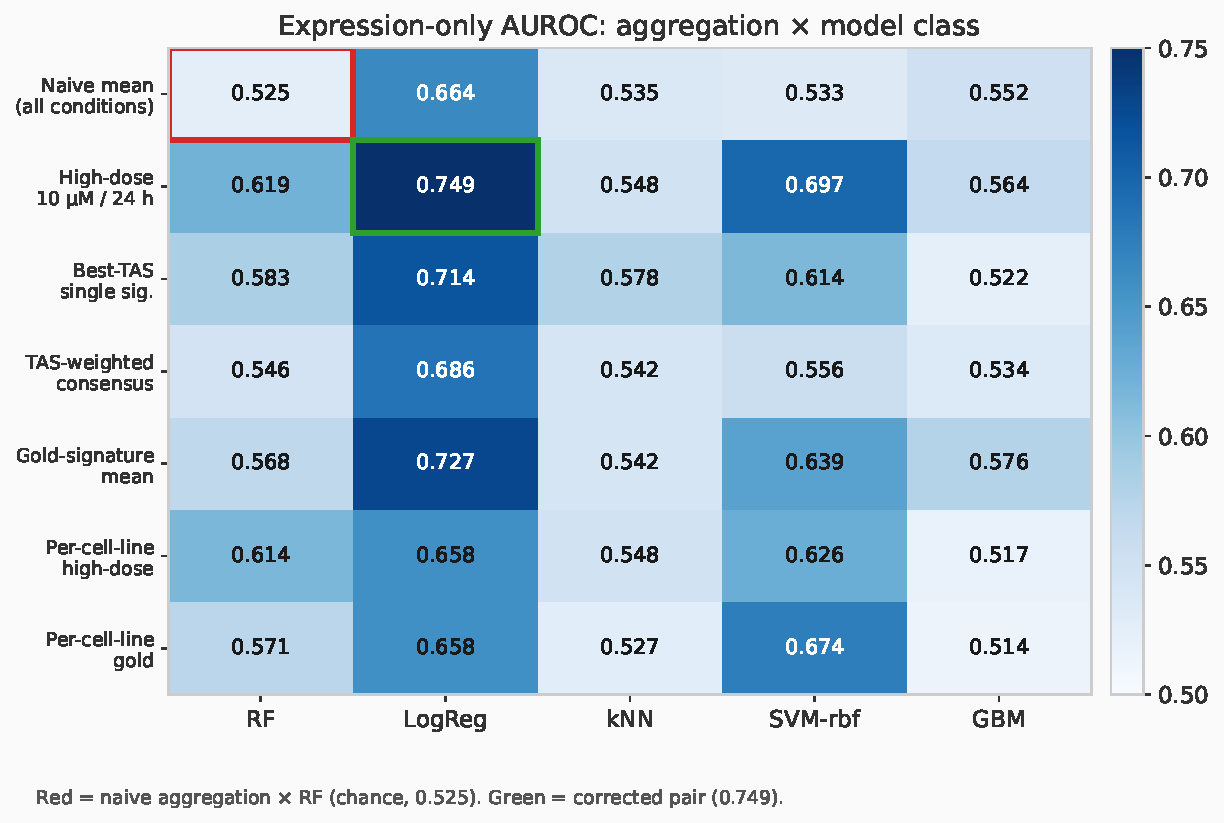
\includegraphics[width=\columnwidth]{../figures/fig1_conjunction.pdf}
\caption{Expression-only AUROC across aggregation strategies $\times$ downstream
model classes (mean over six drug classes, 6 subsampling repeats per cell).
This grid shows the \emph{pattern}; the four corner cells are re-estimated at 30
repeats with bootstrap intervals in Table~\ref{tab:corners}. Neither axis alone explains the
result: the naive-aggregation/random-forest cell (red) is the weakest in the
grid, while correcting both axes (green) is among the strongest. Every other
cell recovers partial signal, so the suppression requires the
\emph{conjunction}.}
\label{fig:grid}
\end{figure}

\begin{figure}[t]
\centering
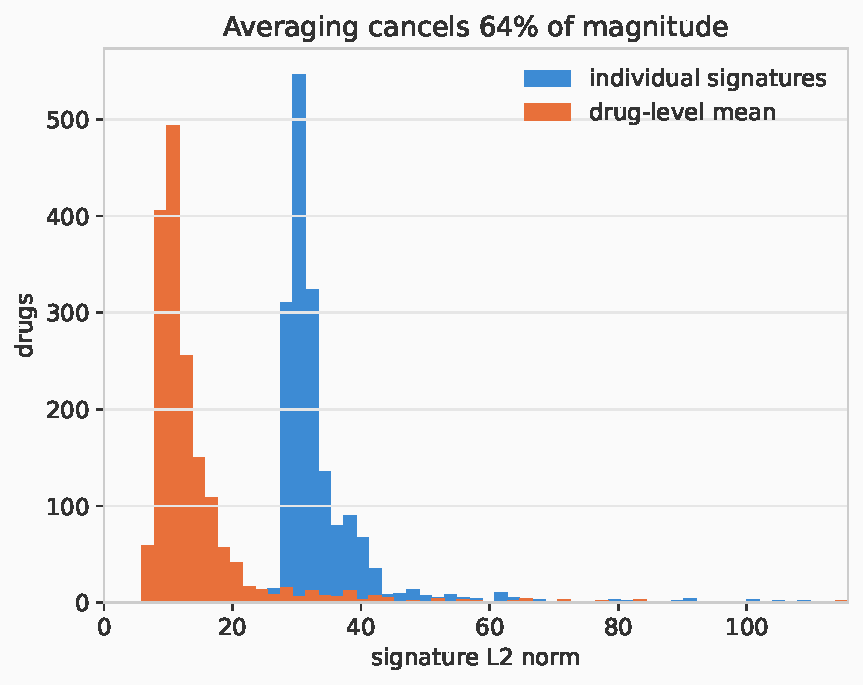
\includegraphics[width=0.9\columnwidth]{../figures/fig3_cancellation.pdf}
\caption{Why naive aggregation destroys signal. Distribution over drugs of the
L2 norm of individual Level-5 signatures (blue) versus the drug-level mean across
all doses, cell lines, and timepoints (orange). Median magnitude falls from
$31.3$ to $11.3$: opposing responses across conditions cancel.}
\label{fig:cancel}
\end{figure}

\textbf{This is probably not unique to us.} Our naive-conjunction estimate
($0.548$) and published raw-signature baselines (e.g.\ TS-978 $=0.507$,
TS-12328 $=0.485$ in MoAble's MoA benchmark) both sit close to chance. We stress
that this is agreement in range only. Our interval does not contain $0.507$, so
we claim just that a near-chance published baseline is consistent with this class
of artifact. Whether any particular published baseline arises from it is beyond
what we can show. Prior
work has separately established that a majority of CMap compounds show weak
transcriptional response and that class recovery for those compounds is close to
random~\cite{sirci2017}, and that L1000 reproducibility depends strongly on
differential-expression strength~\cite{lin2021}. Our result is best read as a
worked example of how preprocessing and model-selection defaults can manufacture
a chance-level baseline where signal exists.

\textbf{A hypothesis we tested and rejected.} Given the above, we hypothesised
that preprocessing choice would dominate model choice in explaining outcome
variance. A variance decomposition over the $7 \times 5$ grid rejects this:
between-model variance accounts for $73.3\%$ of total variance versus $11.5\%$
for between-aggregation, a ratio of $0.16\times$. We report this because we
had intended it as the paper's headline and it did not survive contact with the
data.

\subsection{The corrected features recover known pharmacology}
\label{sec:bio}

A reasonable objection to Section~\ref{sec:f2} is that our ``corrected''
pipeline might simply be overfitting a preprocessing choice to a metric. If the
corrected expression features carry real biology, they should recover known
drug mechanisms without being told what those mechanisms are. They do.

For each class we tested all $978$ landmark genes for a difference in corrected
response between class members and every other compound, using an exact
two-sided Mann-Whitney $U$ test, and kept the ten smallest $p$-values. Classes
hold 5 to 16 compounds against roughly $1{,}700$ others, so the exact null is
the right one; the normal approximation is anti-conservative at these sizes.
For statins the three largest effects among those ten are HMGCS1
($\Delta = +3.66$, $p = 8.1 \times 10^{-5}$), RHOA ($+3.21$,
$9.6 \times 10^{-5}$) and HMGCR ($+2.62$, $3.8 \times 10^{-5}$); a fourth
sterol gene, ELOVL6, also appears ($+1.52$), and the remaining six carry effects
below $|1.8|$. All ten survive Benjamini-Hochberg correction across the 978
genes, at $q \le 0.018$. HMGCR encodes
HMG-CoA reductase, the direct molecular target of every statin, and HMGCS1 sits
immediately upstream in the same sterol-synthesis pathway. RHOA is the third
expected hit rather than a stray one: statins deplete the geranylgeranyl
pyrophosphate that RhoA needs for membrane anchoring. The positive sign is
the expected direction: inhibiting HMGCR relieves sterol-mediated feedback and
drives compensatory SREBP-2 transcription of both genes.

For SSRIs the five smallest $p$-values are EBP ($+1.72$), LIPA ($+1.42$),
TMEM97 ($+1.69$), FDFT1 ($+2.17$) and HMGCS1 ($+3.08$). Four are sterol or
lipid-metabolism genes. The fifth, TMEM97, is the sigma-2 receptor, and EBP is
the sigma-1-associated sterol isomerase; both are established off-target
binding partners of cationic amphiphilic drugs, a class to which most SSRIs
belong. These do not survive correction ($q$ from $0.109$ to $0.257$), so we
read them as a consistency check on the features and not as discoveries.

Neither result was sought. We ran the analysis to characterise the features and
found the canonical target of one class and a documented off-target pathway of
another. This is a positive control on the corrected pipeline, and it is also
the sharpest available evidence that the naive pipeline's chance-level result
was destroying real biological signal rather than reporting its absence.

\section{Independent replication: half the explanation fails}
\label{sec:repl}

A chance-level result invites a strong conclusion, so before drawing one we
tested the explanation on an independent LINCS release. Phase~1 (GSE92742) is a
separate experimental campaign with different cell lines, doses and timepoints.
We extracted the 978 landmark genes for the 46{,}726 Phase~1 signatures covering
1{,}001 of our compounds, and confirmed the extraction with a positive control:
on the corrected Phase~1 features HMGCR sits at $+1.53$ under statins against $+0.13$ elsewhere.

\begin{table}[t]
\centering\small
\caption{The same aggregation and model-class grid on two independent LINCS
releases. Expression-only AUROC, averaged over six drug classes, 6 subsampling
repeats per cell. Phase~1 rows use the nearest available analogue of each
Phase~2 representation. The four Phase~2 cells in the top two rows are
re-estimated at 30 repeats in Table~\ref{tab:corners}.}
\label{tab:repl}
\setlength{\tabcolsep}{3pt}
\begin{tabular}{lcccc}
\toprule
& \multicolumn{2}{c}{Phase 2} & \multicolumn{2}{c}{Phase 1} \\
\cmidrule(lr){2-3}\cmidrule(lr){4-5}
Representation & RF & LogReg & RF & LogReg \\
\midrule
Naive mean, all conditions & 0.525 & 0.664 & 0.580 & \textbf{0.730} \\
High-dose 10\,\textmu M / 24\,h & 0.619 & \textbf{0.749} & 0.543 & 0.686 \\
Strongest single signature & 0.583 & 0.714 & 0.548 & 0.513 \\
Gold / exemplar signature mean & 0.568 & 0.727 & 0.577 & 0.671 \\
\bottomrule
\end{tabular}
\end{table}

\textbf{The model-class effect replicates.} Logistic regression beats random
forest by $+0.09$ to $+0.16$ in seven of the eight release-by-representation
combinations of Table~\ref{tab:repl}. The single exception is the
strongest-signature representation on Phase~1 ($-0.04$), which is also the
weakest representation overall. Whatever else is true, using a tree ensemble on
dense high-dimensional expression features costs roughly $0.14$ AUROC, and it
costs it consistently.

\textbf{The aggregation effect does not replicate, and reverses.} On Phase~2,
restricting to high-dose 24-hour signatures improved matters by $+0.09$ under
both model classes. On Phase~1 the same restriction \emph{hurts}, by $-0.04$
under both, and naive averaging over all conditions is the best representation
tested. Our Phase~2 explanation, that averaging across heterogeneous conditions
destroys signal through cancellation, cannot be the general account: the same
operation on a different release of the same assay is harmless or mildly
beneficial.

We do not have a confident explanation for the reversal. Phase~1 has broader
dose and timepoint coverage per compound, so its naive average may pool more
genuinely replicate measurements and fewer sub-threshold ones. That is a
hypothesis and we have not tested it.

\textbf{What we conclude, narrowly.} Model-class mismatch is a robust hazard for
this modality. Aggregation choice is consequential but release-dependent, and
our chance-level Phase~2 number required both. A practitioner should not read
this paper as saying ``always restrict to high dose''. The transferable
instruction is to treat a near-chance expression baseline as a hypothesis about
the pipeline, then test which part of the pipeline is responsible on their own
data, because the answer differs between releases of the same assay.

This section exists because the replication contradicted us. We had written the
conjunction claim before running it.

\section{Failure 3: correctly specified, the modality is redundant}
\label{sec:f3}

The obvious question is whether a properly specified expression arm becomes
complementary to structure. It does not. With the best model chosen per modality
(structure: RF on ECFP4; expression: logistic regression on high-dose
signatures), a fixed $50{:}50$ probability blend yields:

\begin{center}\small
\setlength{\tabcolsep}{4pt}
\begin{tabular}{lccc}
\toprule
& Structure & Expression & Blend \\
\midrule
Mean AUROC (pooled, $n{=}120$) & 0.9160 & 0.7514 & 0.9173 \\
\bottomrule
\end{tabular}
\end{center}

a gain of $+0.0013$ ($p = 0.15$, $27/120$ wins). Expression carries real signal
($0.751 \gg$ chance) but that signal is largely subsumed by structure for this
task. Per-class gains range from $-0.004$ to $+0.011$ and are individually
non-significant.

\textbf{Replication on a second task family.} Pharmacological class is largely
structure-determined by construction, so we repeated the analysis on SIDER
side-effect prediction, where prior work reports expression outperforming
structure~\cite{wang2016}. With nested (leak-free) blend-weight selection over
$60$ side effects, structure reaches $0.589$, expression $0.530$, and the blend
$0.573$; blending \emph{hurts} ($-0.017$, $p = 1.8\times10^{-4}$).
Gold-signature per-cell-line features, the closest replication
of~\cite{wang2016} we can construct from Phase~2 data, do not change the
ordering: expression reaches $0.543$ on those same endpoints against $0.589$ for
structure. Nor does the independent release. On Phase~1, across $546$ endpoints and $428$ compounds, structure reaches
$0.600$ against $0.512$ for strongest-signature expression features and $0.526$
for exemplar signatures, a deficit of $-0.09$ ($p = 1.4\times10^{-63}$, with
expression ahead on only $87$ of the $546$ endpoints). We did not replicate the published result on either release. We flag
it as an open discrepancy rather than a refutation, since we lack the Phase~1 QC
filtering and the GO-enrichment transform used in that work.

\textbf{One cell where blending does help.} Restricting to transcriptionally
responsive compounds (strongest signature at $\mathrm{TAS} \ge 0.3$, following
Sirci et al.~\cite{sirci2017}) and using gold-signature per-cell-line features,
the fixed blend gains $+0.021$ over structure on drug-class recovery
($p = 0.017$, 40 repeats). We report it because it cuts against our conclusion,
and we do not read much into it. The same cell with a random-forest expression
arm gains $+0.026$ at $p = 0.60$. It is one of a dozen blend comparisons we ran
across representations and compound subsets, so it does not survive correction
for that count. And on SIDER the same restriction with the same features makes
blending worse ($-0.012$, $p = 0.027$). We take the blend gain to be
representation- and task-dependent scatter around zero rather than a recoverable
complementarity.

We also caution that an earlier version of this analysis appeared to show a
$+0.008$ gain; that gain was entirely an artifact of selecting the blend weight
on test predictions, and vanished under nested selection.

\section{Self-audit: five defects, each of which produced a publishable result}
\label{sec:audit}

Over the course of this study we found five defects in our own pipeline. We list
them because each yielded a plausible, presentable result, and because their
interaction is the substantive methodological warning of this paper.

\begin{enumerate}
    \item \textbf{Zero-vector embeddings.} In the class-holdout regime, drug-level
    expression embeddings were aggregated only over signatures visible to that
    regime, so held-out drugs received all-zero embeddings, which are trivially
    separable.
    This produced apparent AUROC of $1.000 \pm 0.000$. Caught only because the
    value was implausibly perfect.

    \item \textbf{Single-seed regime comparison.} The full and class-holdout
    regimes were initially compared at one pretraining seed each, confounding the
    regime effect with seed variance. Fixed by running three seeds per regime.

    \item \textbf{Naive signature aggregation} (Section~\ref{sec:f2}).

    \item \textbf{Mismatched model class for the expression arm}
    (Section~\ref{sec:f2}).

    \item \textbf{Zero-filled representations}, found while preparing the code
    release for this paper. Every aggregation that selects a subset of a
    compound's signatures left an all-zero vector behind for compounds with no
    signature meeting its criterion: 49 of $1{,}725$ for the high-dose subset,
    50 for the gold subset. This is defect~1 again, in a different part of the
    pipeline, and it favoured the random forest, which can split on the
    all-zero pattern: the high-dose random-forest cell fell from $0.641$ to
    $0.619$ once each compound fell back to its own naive mean, while the
    logistic cell rose from $0.733$ to $0.749$. Every number in this paper uses
    the corrected fallback. The conclusions did not change, which is the only
    reason this defect is a footnote rather than a retraction.
\end{enumerate}

Defects 3 and 4 are the instructive pair. Once defect~3 had convinced us that the
modality was uninformative, we then ran five follow-up analyses (a nonlinear
probe, combined raw$+$learned features, an untrained-encoder control, a few-shot
sweep, and a second task family), all of which agreed. They agreed because they
all consumed the same defective features. \emph{Mutual confirmation among analyses
sharing an upstream input is not independent evidence}, and from the outside this
pattern is nearly indistinguishable from a well-controlled negative result. In our
case the error was surfaced by an external prompt to check the domain literature,
which produced an exact numerical match to a known artifact.

\section{Recommendations}
\label{sec:recs}

For practitioners combining chemical structure with L1000 transcriptomics:
(i) do not aggregate Level-5 signatures by unweighted mean across dose, cell line,
and timepoint; prefer high-dose/fixed-timepoint subsets, per-cell-line feature
blocks, or QC-filtered consensus; (ii) select the downstream model class per
modality, as structure and expression have very different geometry;
(iii) treat any expression baseline landing near $0.50$ as a preprocessing
hypothesis to be excluded before it is reported as a modality limit; and
(iv) when several analyses agree, verify that they do not share an upstream
transformation.

For this task family specifically, our results indicate expression is informative
but largely redundant with structure; we do not claim this transfers to tasks
where structure is less determinative, and the unreplicated Wang et al.~\cite{wang2016}
result is a live counterexample worth resolving.

\section{Conclusion}

We tried a standard recipe on real data and it lost to a random forest on
fingerprints in all six disease areas, and to four stronger structural baselines
besides. The interesting part was the diagnosis, and the way it survived only
partially.

Our first explanation, that LINCS expression carries no drug-level signal, was
wrong. Two preprocessing choices produced that number: averaging Level-5
signatures over all experimental conditions, and reusing the structure arm's
model class for the expression arm. On Phase~2 the pair placed the modality at
$0.548$, close enough to chance to read as absence, and correcting both reached
$0.748$.

We then tested that account on an independent release, and half of it failed.
Model-class mismatch costs roughly $0.13$ AUROC in both releases. The
aggregation effect reverses: the restriction that helped on Phase~2 hurts on
Phase~1, where naive averaging is the best representation we tried. We report
this because we had already written the conjunction claim when the replication
contradicted it, and because a paper about pipeline defects that declined to
test its own explanation would be self-refuting.

What survives is narrower and, we think, more useful. Model-class mismatch is a
robust hazard. Aggregation is consequential but release-dependent. A near-chance
expression baseline is a hypothesis about the pipeline before it is a conclusion
about the assay, and which part of the pipeline is responsible has to be
determined on the data at hand rather than assumed from another study.

Correctly specified, the modality remains redundant with structure for these
tasks, so the negative conclusion about cross-modal utility stands even though
the explanation we first gave for it does not.

\section*{Limitations}

\textbf{One published objective, not every published system.}
Section~\ref{sec:published} tests the alignment objective of
Finlayson et al.~\cite{finlayson2021} under our protocol, and it loses in all
six classes. That closes the obvious version of this gap, but not all of it. We
reimplemented their objective with an ECFP4 encoder rather than their Chemprop
D-MPNN, so a graph structure encoder could recover part of the margin, and we
have not run the drug-disease contrastive systems built on knowledge graphs,
which consume different inputs and would need a different evaluation. Our claim
is that two contrastive alignment objectives, one of them the published one,
lose to a random forest on fingerprints under this protocol.

\textbf{One assay.} Results come from LINCS L1000 Phase~2 with replication on
Phase~1 (Section~\ref{sec:repl}), so they generalise across releases but not
beyond the assay. The SIDER replication changes the labels while keeping the same
compounds and measurements, varying the task rather than the data source. Whether
the conjunction reproduces on CMap-independent expression data, or under a
different structural representation, is untested. The Phase~1 QC fields used by
some prior work were unavailable, so the replication uses unfiltered signatures.

\textbf{Small positive classes.} Class sizes of 5--16 drugs bound per-class
power, mitigated by repeated subsampling and by effects consistent across
classes. Membership comes from name matching, not measured efficacy.

\section*{Code and data availability}

Every number in this paper regenerates from the public LINCS releases using the
scripts at \url{https://github.com/edanmn/maidrs-2026-modality}, which also
holds the result log or CSV behind each one and a README mapping every table and
claim to its source. Each figure script prints the values the paper quotes from
it, so those can be checked against a fresh run rather than read off the figure. The raw LINCS releases (GSE70138, GSE92742)
and SIDER 4.1 are public but too large to redistribute; the scripts that build
our dataset from them are included.

\begin{thebibliography}{9}
\bibitem{finlayson2021} S. G. Finlayson, M. B. A. McDermott, A. V. Pickering, S. L. Lipnick, and I. S. Kohane, ``Cross-modal representation alignment of molecular structure and perturbation-induced transcriptional profiles,'' in \emph{Pacific Symposium on Biocomputing}, vol. 26, 2021, pp. 273--284.
\bibitem{radford2021} A. Radford, J. W. Kim, C. Hallacy, A. Ramesh, G. Goh, S. Agarwal, G. Sastry, A. Askell, P. Mishkin, J. Clark, G. Krueger, and I. Sutskever, ``Learning transferable visual models from natural language supervision,'' in \emph{Proc. 38th Int. Conf. Machine Learning}, PMLR 139, 2021, pp. 8748--8763.
\bibitem{wang2020} T. Wang and P. Isola, ``Understanding contrastive representation learning through alignment and uniformity on the hypersphere,'' in \emph{Proc. 37th Int. Conf. Machine Learning}, PMLR 119, 2020, pp. 9929--9939.
\bibitem{sirci2017} F. Sirci, F. Napolitano, S. Pisonero-Vaquero, D. Carrella, D. L. Medina, and D. di Bernardo, ``Comparing structural and transcriptional drug networks reveals signatures of drug activity and toxicity in transcriptional responses,'' \emph{npj Systems Biology and Applications}, vol. 3, p. 23, 2017.
\bibitem{lin2021} N. Lim and P. Pavlidis, ``Evaluation of connectivity map shows limited reproducibility in drug repositioning,'' \emph{Scientific Reports}, vol. 11, no. 1, p. 17624, 2021.
\bibitem{kondadadi2025ctdn} R. Kondadadi, ``Causal temporal diffusion networks for drug repurposing in epilepsy,'' \emph{Briefings in Bioinformatics}, vol. 26, suppl. 1, p. i42, Dec. 2025, conference abstract, doi: 10.1093/bib/bbaf631.074.
\bibitem{wang2016} Z. Wang, N. R. Clark, and A. Ma'ayan, ``Drug-induced adverse events prediction with the LINCS L1000 data,'' \emph{Bioinformatics}, vol. 32, no. 15, pp. 2338--2345, 2016.
\end{thebibliography}

\end{document}
